% Chapter 4

\chapter{Implementation} % Chapter title

\label{ch:implementation} % For referencing the chapter elsewhere, use \autoref{ch:name} 

%---------------------------------------------------------------------------------------- 

From previous chapters, we studied about concepts of a MLS system, as well as logical security policies in the manner of PM.
They together form a list of essential features of a MLS-implemented PMT.
In another world, so far, we had a blueprint of a MLS PMT. 
My \myProject project is built upon this blueprint.
The project's purpose is to evaluate the possibility of my theory and to answer these questions.

\begin{enumerate}
\item How much effort is needed to build a MLS system? 
\item How practically they are used in PM?
\item And how much does it affect to user experience?
\end{enumerate}

In this chapter, we are going to cover the implementation of the project.
It consists of the project's agenda, technical requirements, the program architecture, its data models and their corresponding database schema, relations among data models, etc\dots

%----------------------------------------------------------------------------------------

\section{Project agenda}

\autoref{fig:hotpot_gantchart} is my very first Gant chart of developing time of my project.
Later, although there has been couples of small changes in the time line, however, basically the project finished as scheduled.

\begin{figure}[bth]                                                                                                                                                  
\myfloatalign
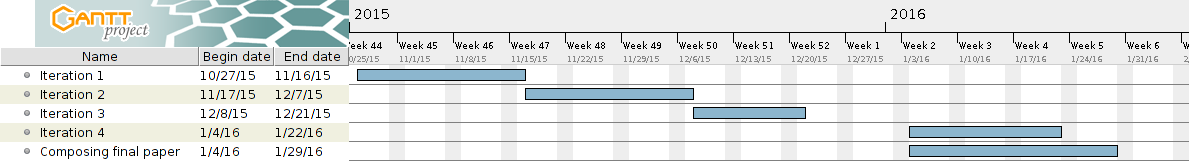
\includegraphics[width=1.0\linewidth]{gfx/chapter_4/hotpot_gantchart}
\caption[HotPot Gant chart]{BLP: HotPot Gant Chart}
\label{fig:hotpot_gantchart}
\end{figure}

The project has four iterations, each of which is three weeks long.

\begin{description}
\item[First iteration]
From 27/10/2015 to 16/11/2015
\begin{itemize}
\item Setup environment. 
\item Create initial DB schema. 
\item Create \emph{account} model with associated details. 
\item Create \emph{project} model. 
\item Add/remove accounts into/from projects. 
\item Create roles, security level. 
\item Assign account to many roles, and one security level.
\end{itemize}

\item[Second iteration]
From 17/11/2015 to 7/12/2015
\begin{itemize}
\item Create \emph{article} model.
\item Assigning security level and role to articles. 
\item Handling user login.
\item List projects related to current logged in account.
\item List articles related to current logged in account.
\end{itemize}

\item[Third iteration]
From 8/12/2015 to 29/12/2015
\begin{itemize}
\item Setup security logic on article actions (\eg create, view, list, edit, delete\dots). 
\item Create \emph{ticket} model. 
\item Apply security logic to ticket actions.
\end{itemize}

\item[Fourth iteration]
From 4/1/2016 to 31/1/2016
\begin{itemize}
\item Fix and update new security logics on \emph{objects' actions}.
\item Implement \emph{directory} structure for managing articles.
\item Apply graphical design.
\item Writing thesis documents and reports.
\end{itemize}
\end{description}
 
Every iterations has one or two days different from the planed schedule, however, in general, the programming part was completed as scheduled.

%----------------------------------------------------------------------------------------

\section{Technical information}

In this section, I am going to introduce about the technologies used in this project, as well as the reason why I chose them at the first place.
The list below are technologies used in the project's developing environment:

\begin{description}
\item[OS] \emph{Ubuntu 14.04}.
It's a free, open source and widely used Linux distro developed by \emph{Canonical Ltd}.
It is easy to use, convenient, and strongly supported by a huge community.
I also used {Vagrant} (\emph{HashiCorp}) and \emph{VirtualBox} (\emph{Oracle}) for virtual environment.
\item[Programming language] \emph{Javascript - Nodejs}.
It's a very dynamic programming language which has an increasing number of developers.
This is my second project using Javascript on back-end, and it's the first project I work with back-end Javascript - Nodejs on my own. It's only for learning purpose, and indeed, I learned many things from this project.
\item[Framework and libraries] \emph{Expressjs, Sequelizejs}.
Expressjs may be the most popular web framework for Nodejs.
It has apparent documentation and a strong community.
Sequelizejs, on the other hand, is a famous and stable DAO library for Nodejs.
\item[Database] \emph{PostgreSQL} is my best choice of SQL Database.
It supports various data types and useful features.
Moreover, it has many libraries to be used in numerous programming language.
\item[Text Editors] \emph{Vim} for coding and \latex for composing thesis papers.
\end{description}

In fact, after finishing developing, I deployed a sample of my project on a cloud machine.
Most of the technical requirements are the same except that I used \emph{CentOS} (\emph{RedHat Inc} instead of Ubuntu for testing purpose and I can confirm that it works on \emph{CentOS} as well.
I can find every things needed on CentOS just like on Ubuntu.

%----------------------------------------------------------------------------------------

\section{Models}

This section is a summary of my project's design.
I utilized MVC design in this project.
All the logical controls will go to \emph{controllers}, which handle all the security policies as previously described in \autoref{ch:background:bell}.
So that, in this thesis document, I only focus explaining about the project's models and their relationship so that we can understand about the system's architecture.

In this section, I am going to list all the data models of the system.
We will learn about their properties, relations which will be illustrated as database diagrams.

%------------------------------------------------

\subsection{Account}

Explain account

%------------------------------------------------

\subsection{Account Detail}

Explain account

%------------------------------------------------

\subsection{Project}

Content

%------------------------------------------------

\subsection{Security Level}

Content

%------------------------------------------------

\subsection{Role}

Content

%------------------------------------------------

\subsection{Article}

Content

%------------------------------------------------

\subsection{Priority}

Content


%------------------------------------------------

\subsection{Ticket}

Content

%----------------------------------------------------------------------------------------

